\documentclass[11pt,a4paper]{article}
\usepackage[T1]{fontenc}
\usepackage[utf8]{inputenc}
\usepackage[french]{babel}
\usepackage{lmodern}
\usepackage{microtype}
\usepackage[margin=2.3cm]{geometry}
\usepackage{graphicx}
\usepackage{booktabs}
\usepackage{float}
\usepackage{caption}
\usepackage{csquotes}
\usepackage[style=numeric-comp,sorting=none,backend=biber,maxbibnames=4]{biblatex}
\usepackage[hidelinks]{hyperref}
\usepackage[french]{cleveref}
\addbibresource{references.bib}
\graphicspath{{../../results/figures/}}
\captionsetup{font=small,labelfont=bf}

\title{Bande L (NISAR) contre bande C (Sentinel-1)\\pour la détection d'une coupe rase dans les Vosges\\[0.4em]
\large Test de faisabilité préparatoire au stage SERTIT / ICube}
\author{Mamadou Galy Diallo}
\date{Novembre 2026}

\begin{document}
\maketitle

\begin{abstract}
\noindent
Ce test compare la capacité de NISAR (bande L, 24~cm) et de Sentinel-1 (bande C, 5,6~cm) à distinguer une
coupe rase récente de la forêt intacte voisine. Le site est une coupe de 2,36~ha réalisée début août 2026 dans le
massif des Vosges, datée et délimitée avec Sentinel-2. Nous utilisons les produits NISAR de niveau~2 produits par
ISCE3 (cohérence GUNW, rétrodiffusion GCOV HH/HV) dans trois géométries, et une série de 13 images Sentinel-1
traitées avec SNAP. Toutes les données sont ramenées sur une grille commune de 20~m. La séparabilité est mesurée
par l'AUC, le d de Cohen et la distance de Jeffries-Matusita, avec des intervalles de confiance par bootstrap par
blocs.
\begin{itemize}
\item \textbf{Cohérence} : en bande L, la paire qui encadre la coupe sépare presque parfaitement coupe et forêt
  (AUC 0,995, cohérence 0,29 contre 0,69), même sur 24~jours. En bande C, la forêt est déjà décorrélée en
  12~jours (0,28) et la cohérence n'apporte presque rien (AUC 0,71--0,74).
\item \textbf{Rétrodiffusion} : la chute en polarisation croisée atteint $-4{,}3$~dB en L (AUC 0,97), contre
  $-2{,}2$~dB en C (AUC 0,91).
\item \textbf{Persistance} : le contraste en bande L persiste jusqu'en novembre, alors que celui de la bande C
  disparaît en octobre.
\end{itemize}
Les quatre hypothèses du cadrage sont confirmées sur ce site. La chaîne de traitement, écrite en modules Python
réutilisables, est directement transposable à la future mission Copernicus en bande L, ROSE-L.
\end{abstract}

\tableofcontents
\newpage

%=====================================================================
\section{Contexte et objectif}

Le stage SERTIT / ICube porte sur l'exploration des bandes L et P (NISAR, BIOMASS) pour la détection de la
déforestation et des glissements de terrain. Depuis 2025, la mission NASA-ISRO NISAR~\cite{kellogg2020nisar,nisar2018handbook}
fournit pour la première fois des données en bande L systématiques, gratuites et ouvertes sur l'Europe. Ses
produits de niveau~2 sont générés par le logiciel ISCE3~\cite{isce3} et distribués par l'ASF~\cite{asf2026nisar}.
En Europe, la bande L sera ensuite assurée par la mission Copernicus ROSE-L, dont le lancement est prévu en
2028~\cite{esa2020rosel}. La bande P (BIOMASS~\cite{quegan2019biomass}) n'acquiert pas sur l'Europe de l'Ouest
(zone d'exclusion SOTR) et reste une perspective.

La détection opérationnelle des coupes et perturbations forestières par radar repose aujourd'hui sur la bande C
de Sentinel-1~\cite{torres2012sentinel1}. Elle exploite la baisse de rétrodiffusion et l'effet d'ombre en bordure de
coupe~\cite{bouvet2018shadow,reiche2021radd}, et la bande L s'est montrée plus sensible à la structure
forestière~\cite{joshi2015mapping}. L'objectif de ce test est de vérifier, sur un cas réel et avec les nouveaux
produits NISAR, si la bande L apporte un gain mesurable par rapport à la bande C pour séparer une coupe rase
récente de la forêt intacte.

\subsection{Question et hypothèses}

\emph{Sur une coupe rase récente des Vosges (juin--novembre 2026), la cohérence interférométrique et la
rétrodiffusion NISAR (bande L) distinguent-elles mieux la coupe de la forêt intacte que Sentinel-1 (bande C) ?}

\begin{description}
\item[H1] En forêt intacte, la cohérence à 12~jours est plus élevée en bande L qu'en bande C : la bande L
  rétrodiffuse sur les troncs et les grosses branches, qui sont stables, alors que la bande C est dominée par le
  feuillage mobile.
\item[H2] L'écart de cohérence entre coupe et forêt est donc plus marqué en bande L.
\item[H3] La baisse de rétrodiffusion après la coupe est plus forte en bande L, car la bande C sature sur forêt
  dense.
\item[H4] La polarisation croisée (HV) est l'indicateur de rétrodiffusion le plus sensible, car elle est liée à la
  diffusion de volume et donc à la biomasse.
\end{description}

%=====================================================================
\section{Données}

L'inventaire du catalogue ASF (\texttt{asf\_search}~\cite{asfsearch}) sur l'emprise Vosges / Alsace, de juin à
novembre 2026, a recensé 546 produits NISAR, dont 93 GCOV et 67 GUNW. Il a aussi recensé 263 images Sentinel-1 IW
SLC réparties sur cinq orbites relatives. Les données utilisées sont résumées au \cref{tab-data}.

\begin{table}[htbp]
\centering\small
\caption{Données utilisées sur le site.}
\label{tab-data}
\begin{tabular}{p{2.6cm}p{5.6cm}p{6.6cm}}
\toprule
Capteur & Produits & Détails \\
\midrule
NISAR (L, 1,26~GHz) & L2 GCOV ($\gamma^0$ HH, HV, RTC) et GUNW (cohérence HH), produits par ISCE3, statut
\emph{provisional} & 3 géométries : A144~F26 et A72~F26 (montantes), D138~F64 (descendante). 10 à 11 GCOV et
8 à 9 GUNW par géométrie, entre le 19/06 et le 10/11/2026. Paires de 12~jours ; la paire qui encadre la coupe fait
24~jours (une acquisition manque fin juillet). \\
Sentinel-1 (C, 5,4~GHz) & IW SLC, VV+VH & Orbite descendante 139, sous-fauchée IW2. 13 dates espacées de 12~jours,
du 14/06 au 06/11/2026 (S1A puis S1C). \\
Sentinel-2~\cite{drusch2012sentinel2} & L2A, NDVI & Référence : délimitation et datation de la coupe (30 dates
claires). \\
ESA WorldCover~\cite{zanaga2022worldcover} & carte 2021, 10~m & Masque forêt. \\
\bottomrule
\end{tabular}
\end{table}

Deux techniques ont réduit le volume à télécharger, qui aurait autrement demandé environ 30~h à 1,8~Mo/s :
\begin{itemize}
\item \textbf{NISAR} : les fichiers HDF5 sont découpés en blocs de $512\times512$ pixels. Nous lisons à distance
  (HTTPS, \texttt{h5py} + \texttt{fsspec}) uniquement les blocs qui couvrent la fenêtre du site, soit environ 15~s
  par couche au lieu de 20~min par fichier.
\item \textbf{Sentinel-1} : le zip distant est lu par requêtes HTTP partielles, et seuls les fichiers de la
  sous-fauchée IW2 sont extraits, soit 1,6~Go au lieu de 4,6~Go par date.
\end{itemize}

%=====================================================================
\section{Site d'étude et référence optique}

Les candidats ont été détectés automatiquement sur deux tuiles Sentinel-2 :
\begin{itemize}
\item critère de changement : NDVI avant $\geq 0{,}7$, dNDVI $\leq -0{,}3$, à l'intérieur du masque forêt ;
\item taille : groupes $\geq 2$~ha ;
\item résultat : 16 candidats, vérifiés ensuite par leurs séries temporelles et par contrôle visuel en couleurs
  vraies et SWIR.
\end{itemize}
La plupart se sont révélés être des dépérissements (scolytes, sécheresse) ou des artefacts (étangs, lisières).
Le site retenu, C11, est une coupe rase de \textbf{2,36~ha} (59 pixels de 20~m) située à 47,910°~N, 6,756°~E,
près du Thillot (haute vallée de la Moselle), au sein d'une forêt continue (\cref{fig-site}).

\begin{figure}[htbp]
\centering
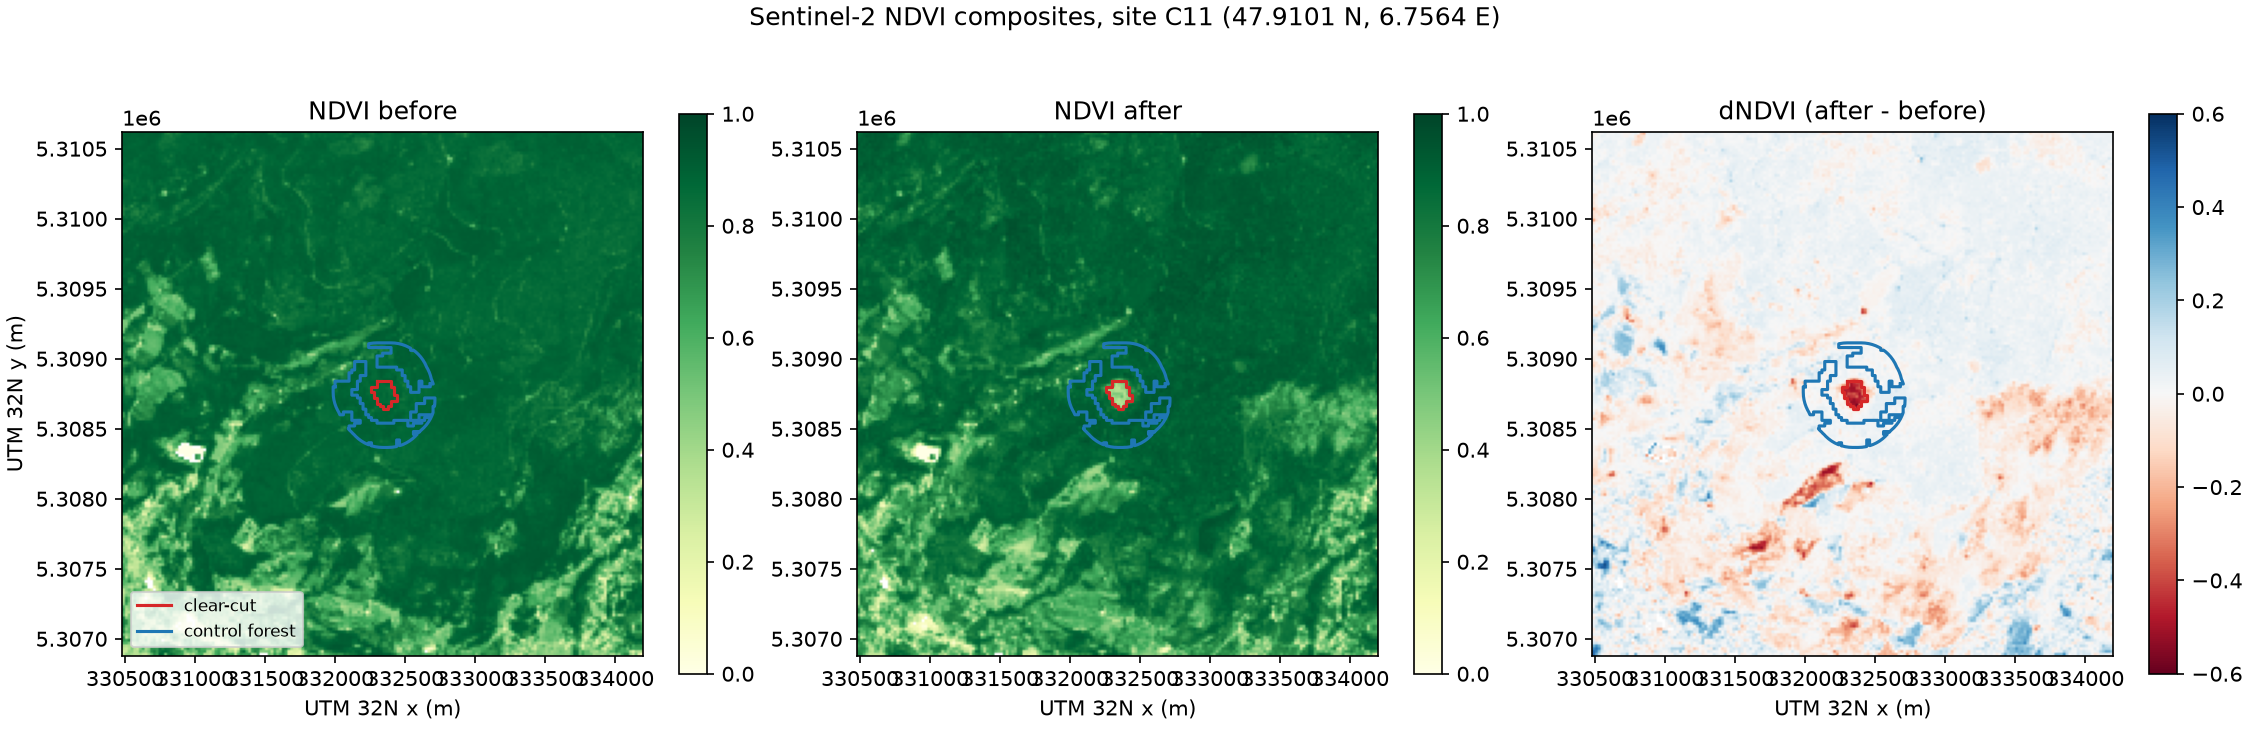
\includegraphics[width=\linewidth]{site_ndvi_maps.png}\\[0.3em]
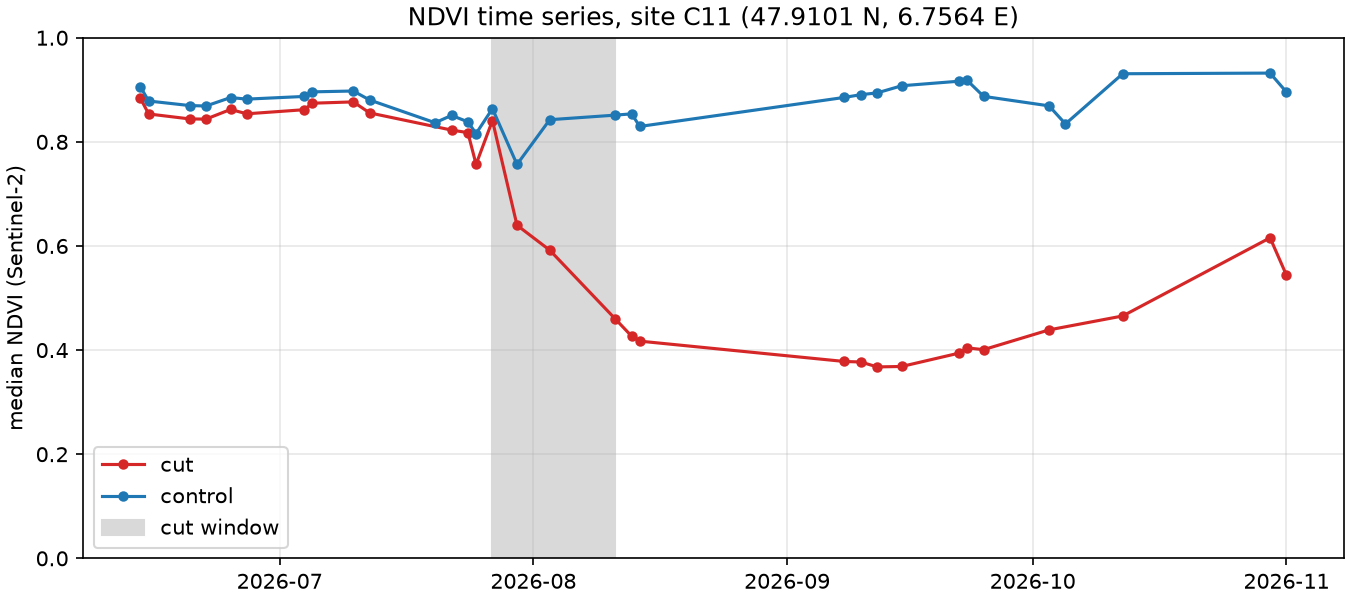
\includegraphics[width=0.85\linewidth]{site_ndvi_timeseries.png}
\caption{Site C11. En haut : NDVI Sentinel-2 avant (juin--juillet), après (septembre--octobre) et différence,
avec la coupe (rouge) et la forêt témoin (bleu). En bas : série NDVI de la coupe et du témoin ; la bande grise
indique la fenêtre de coupe.}
\label{fig-site}
\end{figure}

Le NDVI de la coupe passe de 0,84 (27/07) à 0,42--0,46 (11--13/08) ; celui du témoin reste stable (0,85--0,92).
\begin{itemize}
\item \textbf{Fenêtre de coupe} : nous retenons la fenêtre prudente du 27/07 au 11/08.
\item \textbf{Forêt témoin} : anneau de forêt intacte de 100 à 275~m autour de la coupe (548 pixels, 21,8~ha),
  qui partage le versant, l'altitude et le peuplement de la coupe. La marge de 100~m évite les effets de lisière.
\end{itemize}

%=====================================================================
\section{Méthodes}

\subsection{Chaîne de traitement}

\paragraph{NISAR.} Les produits L2 sont utilisés tels que livrés par ISCE3 :
\begin{itemize}
\item $\gamma^0$ HH et HV du GCOV, déjà corrigés du relief (RTC~\cite{small2011flattening}) ;
\item cohérence HH du GUNW, dans la couche \texttt{wrappedInterferogram} à 20~m et dans la couche
  \texttt{unwrappedInterferogram} à 80~m.
\end{itemize}
Le GUNW n'existe qu'en co-polarisation : l'information HV ne vient que du GCOV.

\paragraph{Sentinel-1.} Deux graphes SNAP~\cite{snap} (\texttt{gpt}), versionnés dans le dépôt, sont appliqués :
\begin{itemize}
\item \textbf{$\gamma^0$} : TOPSAR-Split, orbites précises, suppression du bruit thermique, calibration $\beta^0$, débursting,
  multivue $4\times1$, Terrain-Flattening, puis géocodage à 20~m (UTM 32N, MNT Copernicus 30~m).
\item \textbf{Cohérence} : Back-Geocoding, estimation sur une fenêtre $10\times3$ après soustraction des phases
  plate et topographique, débursting, puis géocodage à 20~m. L'étape ESD est omise car le site tient dans un seul
  burst (sans recouvrement, l'ESD donne une cohérence nulle).
\end{itemize}

\paragraph{Grille commune.} Toutes les couches sont rééchantillonnées sur une grille de 20~m en UTM~32N couvrant
le site plus 1,5~km :
\begin{itemize}
\item $\gamma^0$ NISAR : moyenne en puissance linéaire ;
\item cohérence NISAR à 20~m : moyenne ;
\item Sentinel-1 : interpolation bilinéaire.
\end{itemize}
Les $\gamma^0$ sont ensuite convertis en dB.

\subsection{Variables de changement}

Chaque acquisition est classée par rapport à la fenêtre de coupe :
\begin{itemize}
\item \emph{avant} : image, ou paire de cohérence, entièrement antérieure au 27/07 ;
\item \emph{après} : entièrement postérieure au 11/08 ;
\item \emph{à cheval} : paire qui encadre la coupe.
\end{itemize}
Les paires avant et après sont limitées à 12--13~jours. La paire à cheval peut atteindre 25~jours, pour
inclure la paire NISAR de 24~jours.

Variables par capteur et par géométrie :
\begin{itemize}
\item $\Delta\gamma^0$ : $\gamma^0$ moyen après $-$ $\gamma^0$ moyen avant (dB), et $\gamma^0$ après ;
\item cohérence de la paire à cheval sur la coupe ;
\item chute de cohérence : paire à cheval $-$ cohérence avant ;
\item $\Delta$ cohérence : cohérence après $-$ cohérence avant.
\end{itemize}

\subsection{Mesures de séparabilité et de détection}

Pour chaque variable, nous comparons les pixels de la coupe ($a$) à ceux du témoin ($b$) avec :
\begin{itemize}
\item l'écart des moyennes $\Delta=\bar a-\bar b$ ;
\item le d de Cohen~\cite{cohen1988power} ;
\item l'aire sous la courbe ROC (AUC, statistique de Mann-Whitney~\cite{hanley1982auc}), exprimée comme
  $\max(\mathrm{AUC}, 1-\mathrm{AUC})$ (0,5 : aucune séparation ; 1 : séparation parfaite) ;
\item la distance de Jeffries-Matusita~\cite{swain1978remote} (0 à 2).
\end{itemize}
Les pixels voisins sont spatialement corrélés, ce qui rendrait les p-valeurs trompeuses. Les intervalles de
confiance à 95~\% de l'AUC sont donc obtenus par bootstrap par blocs~\cite{kunsch1989bootstrap}, en rééchantillonnant
des blocs de $3\times3$ pixels (60~m ; $5\times5$ pour les couches à 80~m), 300 tirages.

\paragraph{Prototype de détection.} Chaque variable est aussi évaluée comme détecteur sur toute la fenêtre
($188\times187$ pixels, $3{,}7\times3{,}7$~km) :
\begin{itemize}
\item \textbf{référence} : dNDVI Sentinel-2 $\leq -0{,}3$ sur forêt (NDVI avant $\geq 0{,}7$), les changements
  partiels ambigus étant exclus. Elle compte 95 pixels coupés sur 25\,723, soit 0,4~\% ;
\item \textbf{scores} : AUC sur la fenêtre, F1 au seuil d'Otsu~\cite{otsu1979threshold} et F1 maximal.
\end{itemize}

\paragraph{Contrôles.}
\begin{itemize}
\item Avant la coupe, la coupe et le témoin doivent être indiscernables.
\item Une analyse de sensibilité répète tout le calcul avec des polygones érodés de 20~m, ce qui laisse 25 pixels
  de coupe \enquote{purs}.
\end{itemize}

%=====================================================================
\section{Résultats}

\subsection{Contrôle avant la coupe}

Sur les acquisitions antérieures à la coupe, l'AUC entre coupe et témoin vaut 0,51 à 0,62 selon le capteur et la
variable : les deux zones sont radiométriquement et interférométriquement équivalentes avant la coupe. Ce contrôle
valide le choix du témoin : les écarts mesurés ensuite sont attribuables à la coupe.

\subsection{Séparabilité des variables de changement}

Le \cref{tab-core} compare les variables communes aux deux capteurs, et la \cref{fig-auc} classe toutes les
variables. Le \cref{tab-best} donne la meilleure variable à 20~m par capteur et par géométrie.

\begin{table}[htbp]
\centering
\scriptsize
\caption{Variables comparables entre capteurs (20 m) : variation de $\gamma^0$, cohérence de la paire qui encadre la coupe et variation de cohérence (après $-$ avant).}
\label{tab-core}
\begin{tabular}{llcrrlrrr}
\toprule
Capteur & Variable & $n_{av}/n_{ap}$ & $\Delta$ & $d$ & AUC [IC 95\,\%] & JM & AUC fen. & F1$_{max}$ \\
\midrule
NISAR A144F26 & cohérence de la paire sur la coupe HH & 2/6 & $-$0{,}40 & $-$3{,}9 & 1{,}00 [0{,}99--1{,}00] & 1{,}76 & 0{,}87 & 0{,}09 \\
NISAR A144F26 & $\Delta\gamma^0$ après $-$ avant (dB) HV & 3/8 & $-$4{,}25 & $-$3{,}7 & 0{,}97 [0{,}93--0{,}99] & 1{,}28 & 0{,}84 & 0{,}27 \\
NISAR A144F26 & $\Delta\gamma^0$ après $-$ avant (dB) HH & 3/8 & $-$4{,}22 & $-$3{,}2 & 0{,}96 [0{,}93--0{,}99] & 1{,}09 & 0{,}80 & 0{,}24 \\
NISAR A144F26 & $\Delta$ cohérence après $-$ avant HH & 2/6 & $-$0{,}08 & $-$1{,}1 & 0{,}77 [0{,}66--0{,}85] & 0{,}27 & 0{,}67 & 0{,}08 \\
\addlinespace
NISAR A72F26 & $\Delta\gamma^0$ après $-$ avant (dB) HV & 3/7 & $-$3{,}72 & $-$3{,}0 & 0{,}94 [0{,}89--0{,}99] & 1{,}04 & 0{,}78 & 0{,}27 \\
NISAR A72F26 & $\Delta\gamma^0$ après $-$ avant (dB) HH & 3/7 & $-$2{,}96 & $-$2{,}3 & 0{,}92 [0{,}86--0{,}97] & 0{,}82 & 0{,}78 & 0{,}22 \\
NISAR A72F26 & cohérence de la paire sur la coupe HH & 3/5 & $-$0{,}25 & $-$1{,}8 & 0{,}91 [0{,}85--0{,}96] & 0{,}82 & 0{,}80 & 0{,}07 \\
NISAR A72F26 & $\Delta$ cohérence après $-$ avant HH & 3/5 & $-$0{,}05 & $-$0{,}7 & 0{,}65 [0{,}51--0{,}82] & 0{,}15 & 0{,}56 & 0{,}05 \\
\addlinespace
NISAR D138F64 & cohérence de la paire sur la coupe HH & 1/5 & $-$0{,}31 & $-$3{,}7 & 1{,}00 [0{,}99--1{,}00] & 1{,}72 & 0{,}89 & 0{,}10 \\
NISAR D138F64 & $\Delta\gamma^0$ après $-$ avant (dB) HV & 2/7 & $-$2{,}33 & $-$1{,}5 & 0{,}84 [0{,}78--0{,}89] & 0{,}44 & 0{,}71 & 0{,}14 \\
NISAR D138F64 & $\Delta\gamma^0$ après $-$ avant (dB) HH & 2/7 & $-$1{,}69 & $-$1{,}1 & 0{,}72 [0{,}60--0{,}84] & 0{,}29 & 0{,}64 & 0{,}11 \\
NISAR D138F64 & $\Delta$ cohérence après $-$ avant HH & 1/5 & $-$0{,}01 & $-$0{,}1 & 0{,}55 [0{,}50--0{,}67] & 0{,}05 & 0{,}54 & 0{,}03 \\
\addlinespace
Sentinel-1 T139 & $\Delta\gamma^0$ après $-$ avant (dB) VH & 4/8 & $-$2{,}20 & $-$2{,}1 & 0{,}91 [0{,}85--0{,}94] & 0{,}72 & 0{,}79 & 0{,}14 \\
Sentinel-1 T139 & $\Delta\gamma^0$ après $-$ avant (dB) VV & 4/8 & $-$2{,}53 & $-$2{,}4 & 0{,}90 [0{,}82--0{,}95] & 0{,}76 & 0{,}87 & 0{,}22 \\
Sentinel-1 T139 & cohérence de la paire sur la coupe VH & 3/7 & $-$0{,}06 & $-$0{,}8 & 0{,}74 [0{,}68--0{,}80] & 0{,}40 & 0{,}67 & 0{,}01 \\
Sentinel-1 T139 & cohérence de la paire sur la coupe VV & 3/7 & $-$0{,}06 & $-$0{,}8 & 0{,}71 [0{,}60--0{,}80] & 0{,}17 & 0{,}63 & 0{,}04 \\
Sentinel-1 T139 & $\Delta$ cohérence après $-$ avant VV & 3/7 & 0{,}06 & 0{,}7 & 0{,}70 [0{,}59--0{,}78] & 0{,}13 & 0{,}66 & 0{,}02 \\
Sentinel-1 T139 & $\Delta$ cohérence après $-$ avant VH & 3/7 & 0{,}03 & 0{,}5 & 0{,}65 [0{,}55--0{,}73] & 0{,}11 & 0{,}61 & 0{,}01 \\
\bottomrule
\end{tabular}
\end{table}


\begin{figure}[p]
\centering
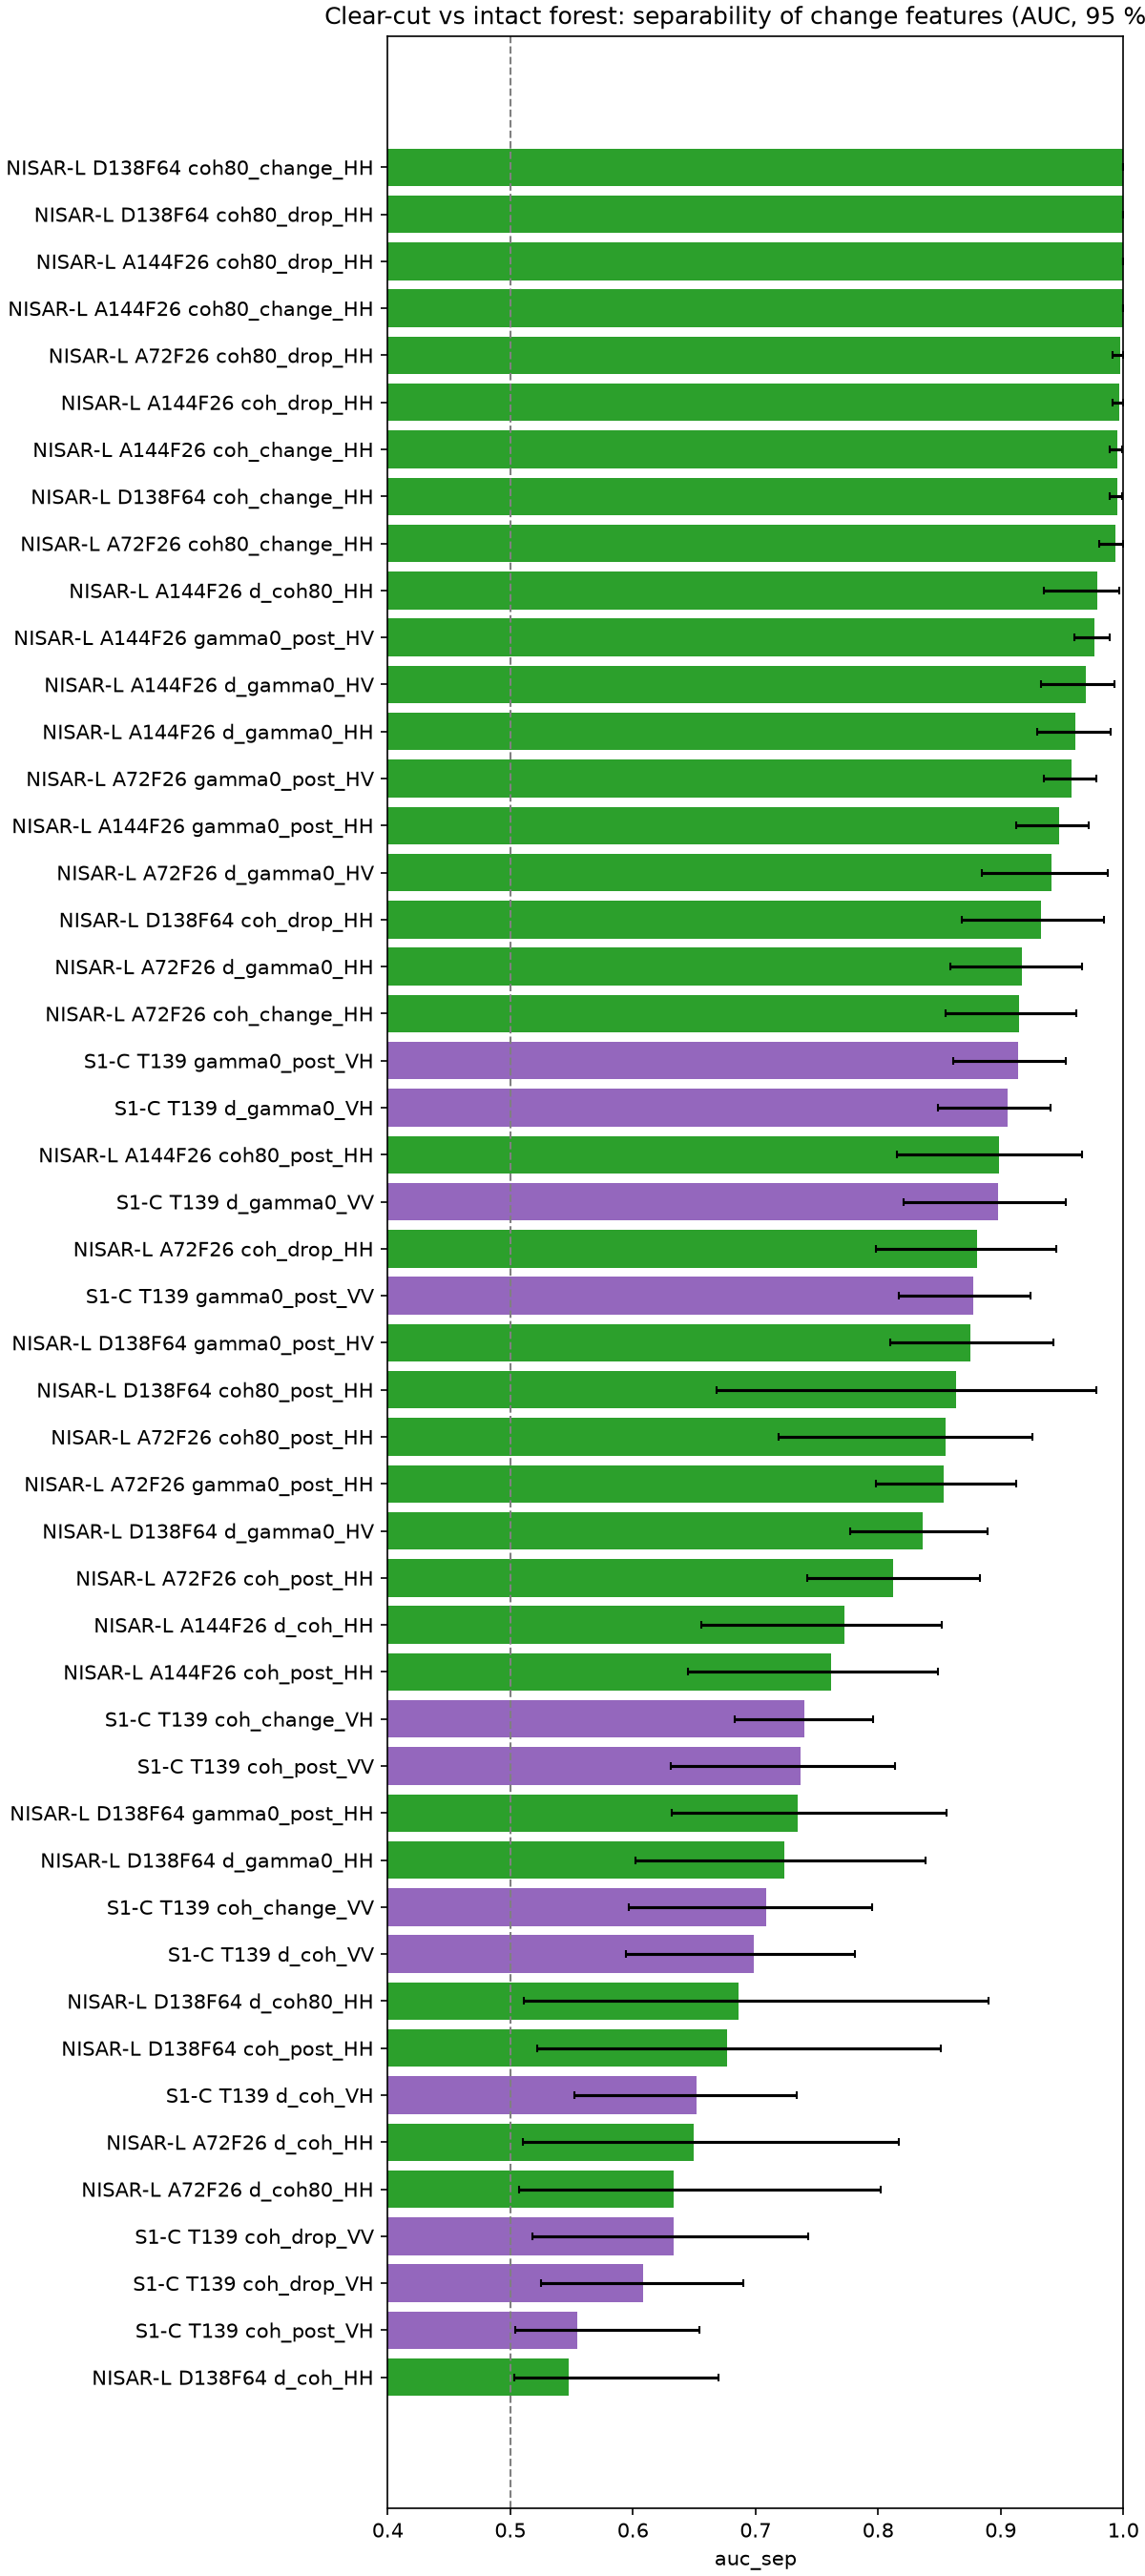
\includegraphics[height=0.92\textheight]{comparison_auc.png}
\caption{AUC de séparation coupe / témoin de toutes les variables de changement, avec l'intervalle de confiance à
95~\% (bootstrap par blocs). Vert : NISAR (bande L) ; violet : Sentinel-1 (bande C). Les variables
\texttt{coh80} sont à 80~m et ne contiennent qu'environ 4 pixels indépendants dans la coupe.}
\label{fig-auc}
\end{figure}

\begin{table}[htbp]
\centering
\scriptsize
\caption{Meilleure variable à 20 m par capteur et géométrie.}
\label{tab:best}
\begin{tabular}{llcrrlrrr}
\toprule
Capteur & Variable & $n_{av}/n_{ap}$ & $\Delta$ & $d$ & AUC [IC 95\,\%] & JM & AUC fen. & F1$_{max}$ \\
\midrule
NISAR A144F26 & chute de cohérence (paire sur la coupe $-$ avant) HH & 2/6 & $-$0{,}42 & $-$4{,}6 & 1{,}00 [0{,}99--1{,}00] & 1{,}82 & 0{,}82 & 0{,}29 \\
\addlinespace
NISAR D138F64 & cohérence de la paire sur la coupe HH & 1/5 & $-$0{,}31 & $-$3{,}7 & 1{,}00 [0{,}99--1{,}00] & 1{,}72 & 0{,}89 & 0{,}10 \\
\addlinespace
NISAR A72F26 & $\gamma^0$ après (dB) HV & 3/7 & $-$3{,}56 & $-$2{,}3 & 0{,}96 [0{,}94--0{,}98] & 1{,}12 & 0{,}92 & 0{,}06 \\
\addlinespace
Sentinel-1 T139 & $\gamma^0$ après (dB) VH & 4/8 & $-$2{,}27 & $-$1{,}7 & 0{,}91 [0{,}86--0{,}95] & 0{,}67 & 0{,}86 & 0{,}04 \\
\bottomrule
\end{tabular}
\end{table}


\paragraph{Cohérence.} C'est la différence la plus nette entre les deux bandes.
\begin{itemize}
\item \textbf{Bande L} : sur la paire de 24~jours qui encadre la coupe, la cohérence NISAR vaut 0,26--0,33 dans la
  coupe, contre 0,50--0,69 dans la forêt témoin. L'AUC atteint 0,995 en A144 et en D138, avec un d de Cohen
  inférieur à $-3{,}7$.
\item \textbf{Bande C} : la forêt est déjà décorrélée en 12~jours (cohérence moyenne 0,28). La paire Sentinel-1 qui
  encadre la coupe ne la distingue que faiblement ($\Delta=-0{,}06$, AUC 0,71--0,74).
\item \textbf{Après la coupe} : la différence de cohérence entre coupe et forêt redevient faible dans les deux
  bandes (AUC 0,55--0,77). C'est donc \emph{l'événement} de coupe, et non l'état final, que la cohérence capte.
\end{itemize}

\paragraph{Rétrodiffusion.} Les deux bandes détectent la coupe, mais la bande L plus fortement.
\begin{itemize}
\item En polarisation croisée, la chute atteint $-4{,}3$~dB en A144 (AUC 0,97) et $-3{,}7$~dB en A72 (AUC 0,94).
  En VH Sentinel-1, elle est de $-2{,}2$~dB (AUC 0,91).
\item En co-polarisation, on mesure $-4{,}2$~dB en HH (AUC 0,96) contre $-2{,}5$~dB en VV (AUC 0,90).
\item La géométrie descendante NISAR D138 est nettement moins discriminante ($-2{,}3$~dB en HV, AUC 0,84).
\end{itemize}

\subsection{Évolution temporelle et persistance du contraste}

Les \cref{fig-tsL,fig-tsC} montrent les séries temporelles de la coupe et du témoin, et la \cref{fig-persist} l'AUC
de séparation date par date.
\begin{itemize}
\item \textbf{Bande L} : le $\gamma^0$ HV de la coupe chute brutalement de $-9{,}2$ à $-13{,}7$~dB et reste à ce niveau
  jusqu'en novembre ; le témoin, lui, reste stable à $-9{,}2$~dB.
\item \textbf{Bande C} : la baisse est visible en août et septembre, puis la coupe remonte au niveau de la forêt en
  octobre (AUC VH 0,52 le 25/10).
\end{itemize}
Le \cref{tab-persistence} quantifie ce comportement : entre août--septembre et octobre--novembre, l'AUC HV de NISAR
A144 passe seulement de 0,95 à 0,91, alors que l'AUC VV de Sentinel-1 passe de 0,86 à 0,66.

\begin{figure}[htbp]
\centering
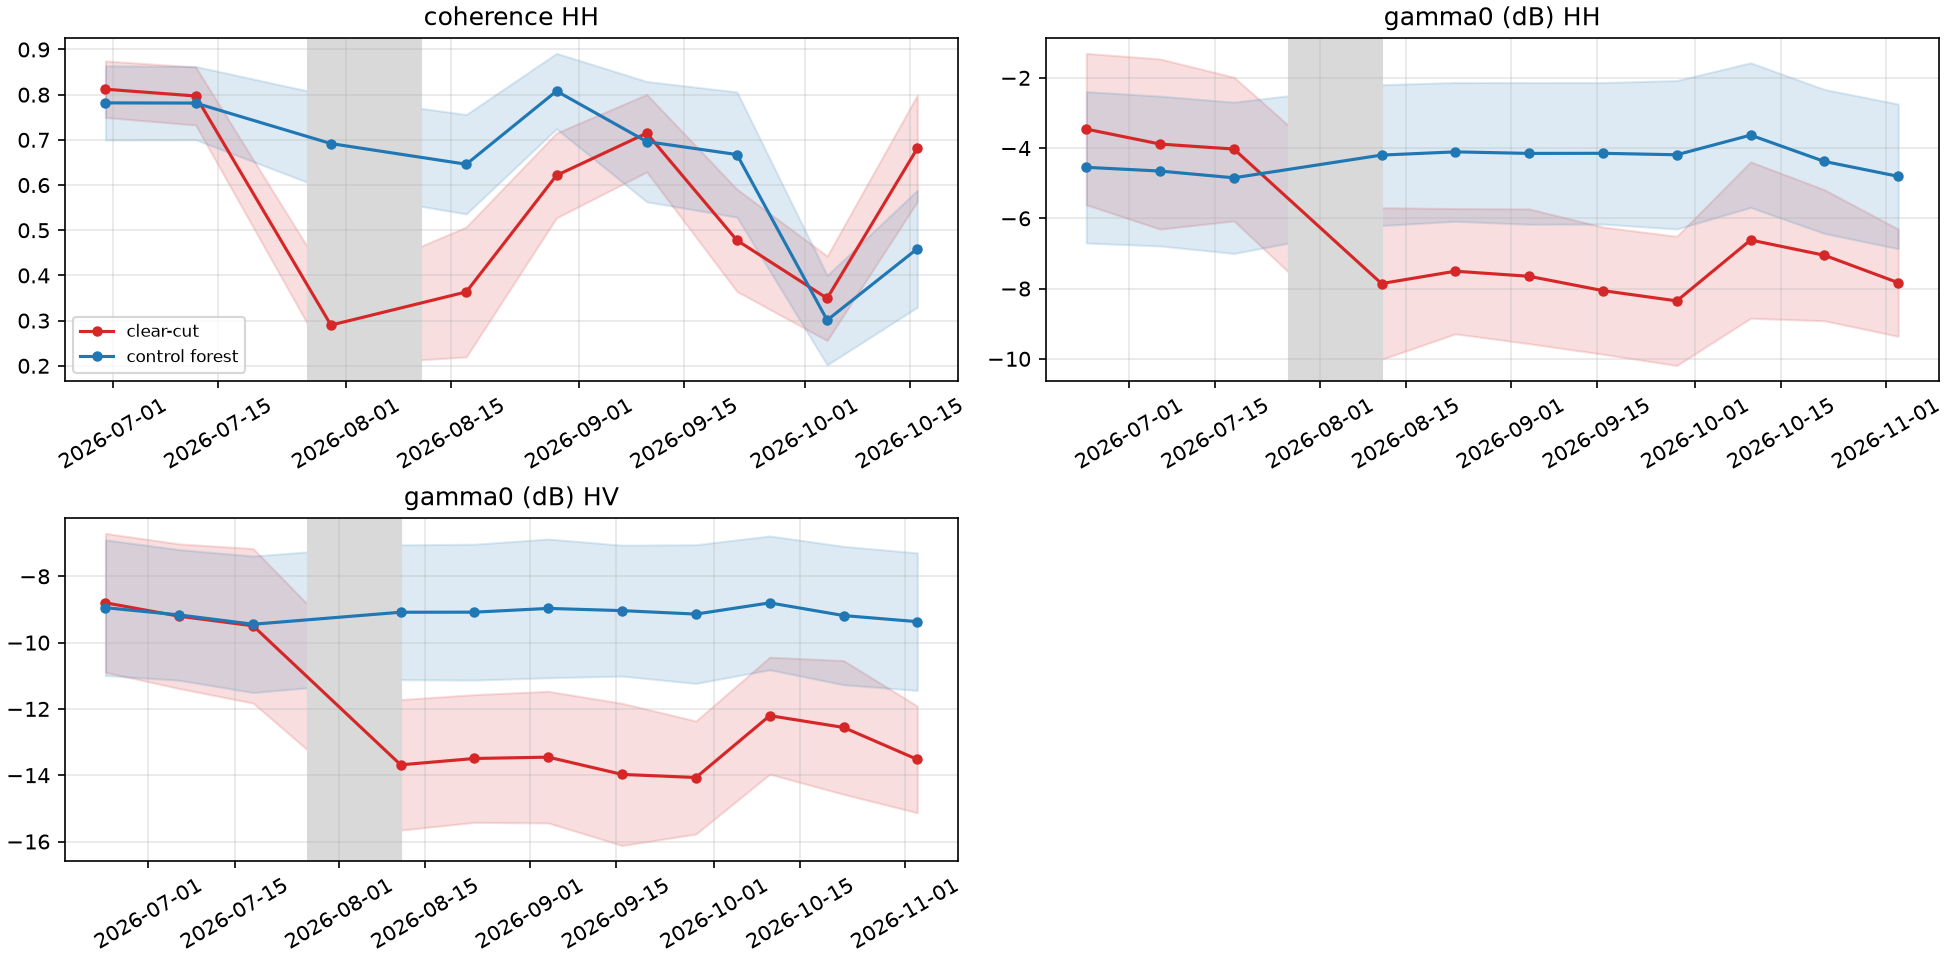
\includegraphics[width=\linewidth]{comparison_ts_NISAR-L_A144F26.png}
\caption{NISAR A144 : cohérence HH (paires placées à leur date médiane), $\gamma^0$ HH et HV de la coupe (rouge) et du
témoin (bleu), moyenne $\pm$ écart-type ; la bande grise indique la fenêtre de coupe.}
\label{fig-tsL}
\end{figure}

\begin{figure}[htbp]
\centering
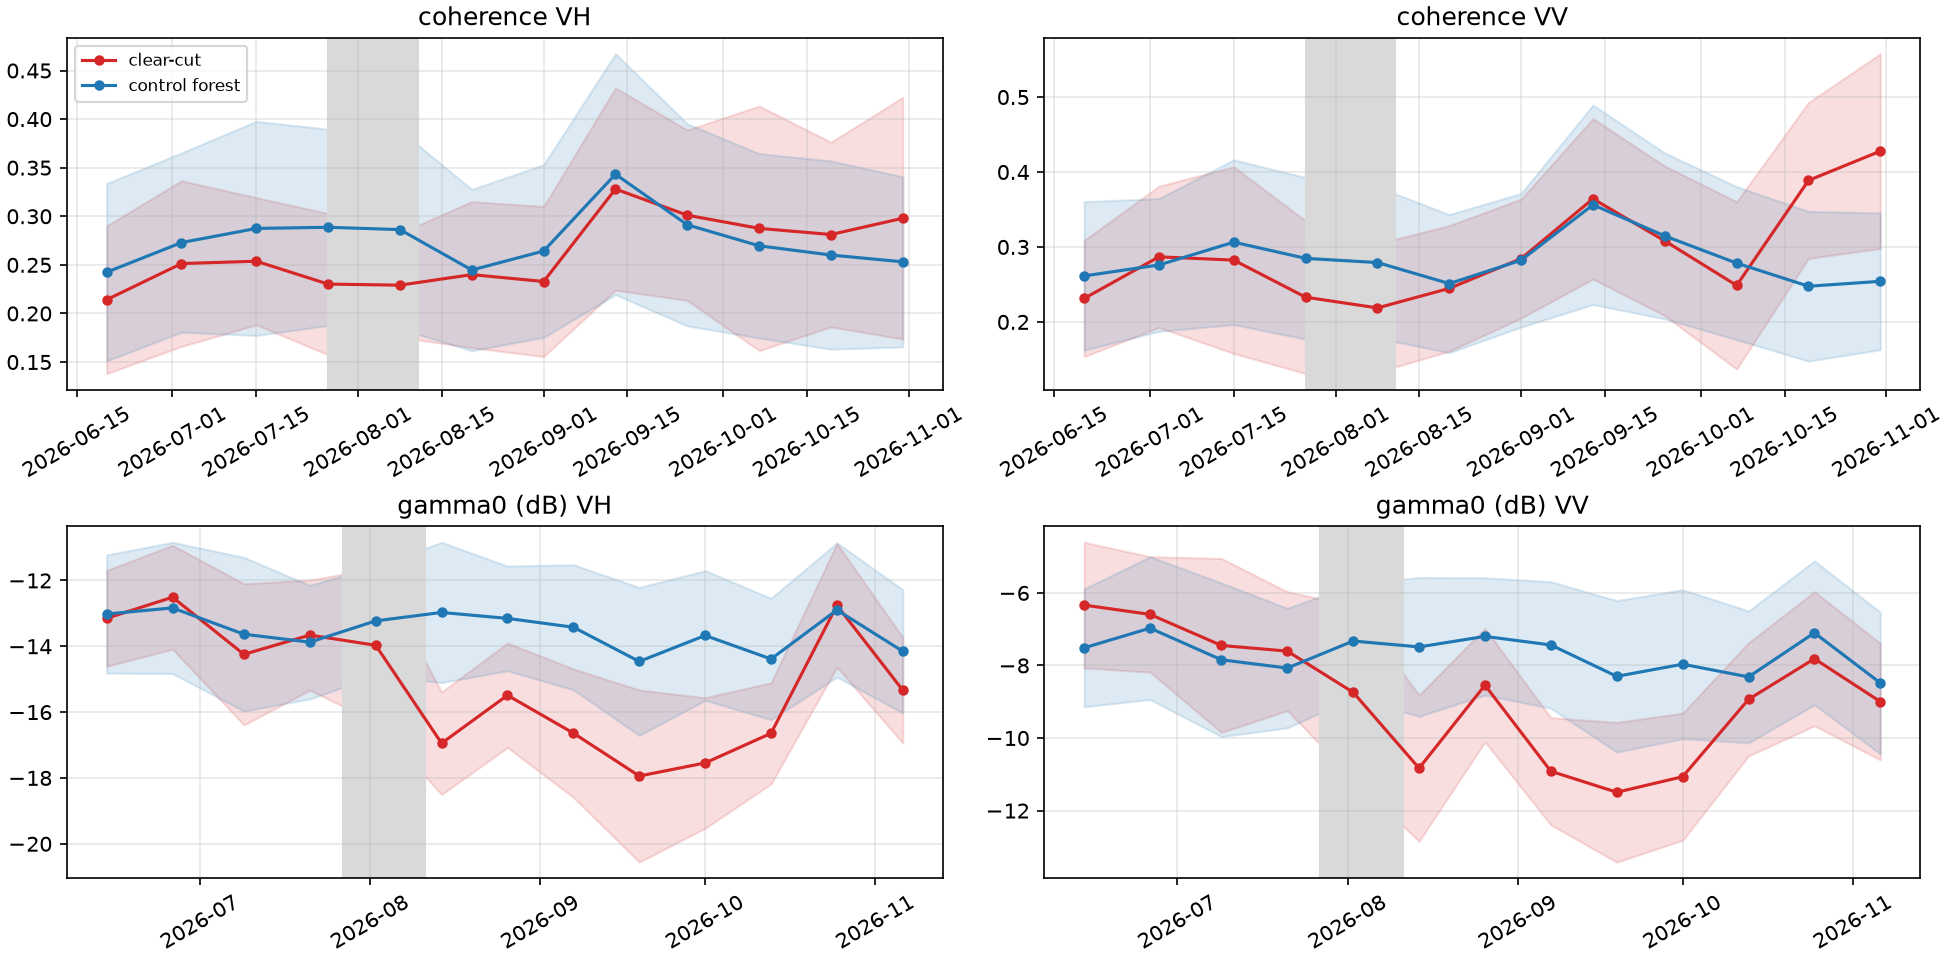
\includegraphics[width=\linewidth]{comparison_ts_S1-C_T139.png}
\caption{Sentinel-1 orbite 139 : cohérence VH et VV, $\gamma^0$ VH et VV de la coupe (rouge) et du témoin (bleu).}
\label{fig-tsC}
\end{figure}

\begin{figure}[htbp]
\centering
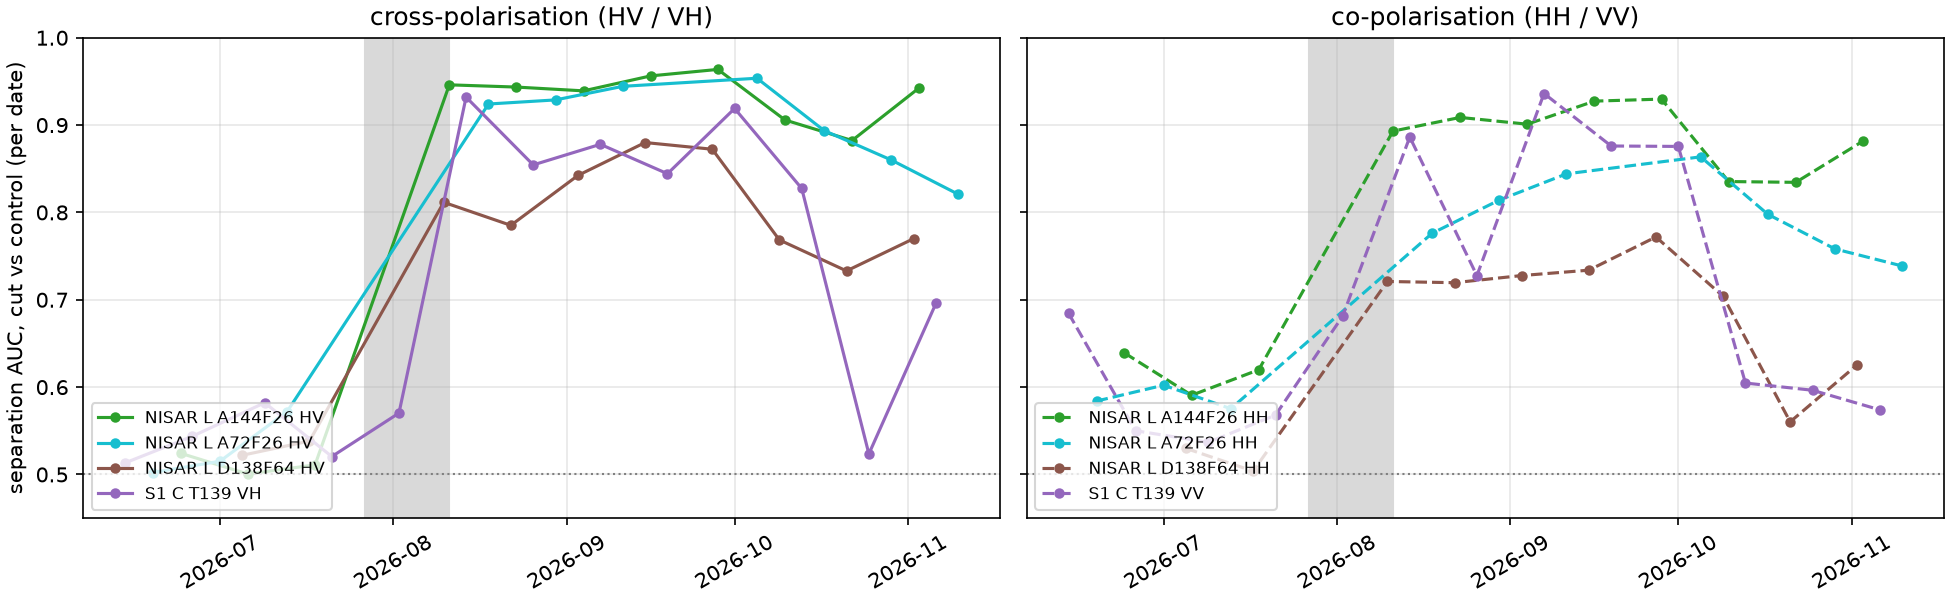
\includegraphics[width=\linewidth]{comparison_persistence.png}
\caption{AUC de séparation coupe / témoin date par date pour la rétrodiffusion, en polarisation croisée (à gauche)
et en co-polarisation (à droite). Le contraste reste élevé en bande L et s'effondre en octobre en bande C.}
\label{fig-persist}
\end{figure}

\begin{table}[htbp]
\centering
\small
\caption{Persistance du contraste de rétrodiffusion après la coupe : AUC de séparation et écart coupe $-$ témoin, moyennés par date sur deux périodes.}
\label{tab:persistence}
\begin{tabular}{llrrrr}
\toprule
Capteur & Pol. & AUC août--sept. & $\Delta$ (dB) & AUC oct.--nov. & $\Delta$ (dB) \\
\midrule
NISAR A144F26 & HH & 0{,}91 & $-$3{,}7 & 0{,}85 & $-$2{,}9 \\
NISAR A144F26 & HV & 0{,}95 & $-$4{,}7 & 0{,}91 & $-$3{,}6 \\
NISAR A72F26 & HH & 0{,}81 & $-$2{,}6 & 0{,}79 & $-$2{,}3 \\
NISAR A72F26 & HV & 0{,}93 & $-$4{,}2 & 0{,}88 & $-$3{,}3 \\
NISAR D138F64 & HH & 0{,}74 & $-$2{,}0 & 0{,}63 & $-$1{,}0 \\
NISAR D138F64 & HV & 0{,}84 & $-$2{,}9 & 0{,}76 & $-$2{,}1 \\
Sentinel-1 T139 & VH & 0{,}88 & $-$3{,}3 & 0{,}74 & $-$1{,}8 \\
Sentinel-1 T139 & VV & 0{,}86 & $-$2{,}8 & 0{,}66 & $-$1{,}2 \\
\bottomrule
\end{tabular}
\end{table}


\subsection{Cartes et prototype de détection}

La \cref{fig-maps} montre les cartes de changement sur le voisinage du site. La coupe ressort nettement en
$\Delta\gamma^0$ HV et en cohérence NISAR, ainsi qu'en $\Delta\gamma^0$ VH Sentinel-1, mais pas en cohérence
Sentinel-1.

Sur toute la fenêtre, l'AUC de détection atteint 0,93 pour le $\gamma^0$ HV NISAR après la coupe, et 0,86--0,87 pour le
$\gamma^0$ Sentinel-1. Le F1 reste en revanche faible (F1 maximal de 0,29 au mieux) : la coupe ne représente que 0,4~\%
des pixels, et un seuil sur une seule variable produit inévitablement de nombreuses fausses alarmes.

\begin{figure}[htbp]
\centering
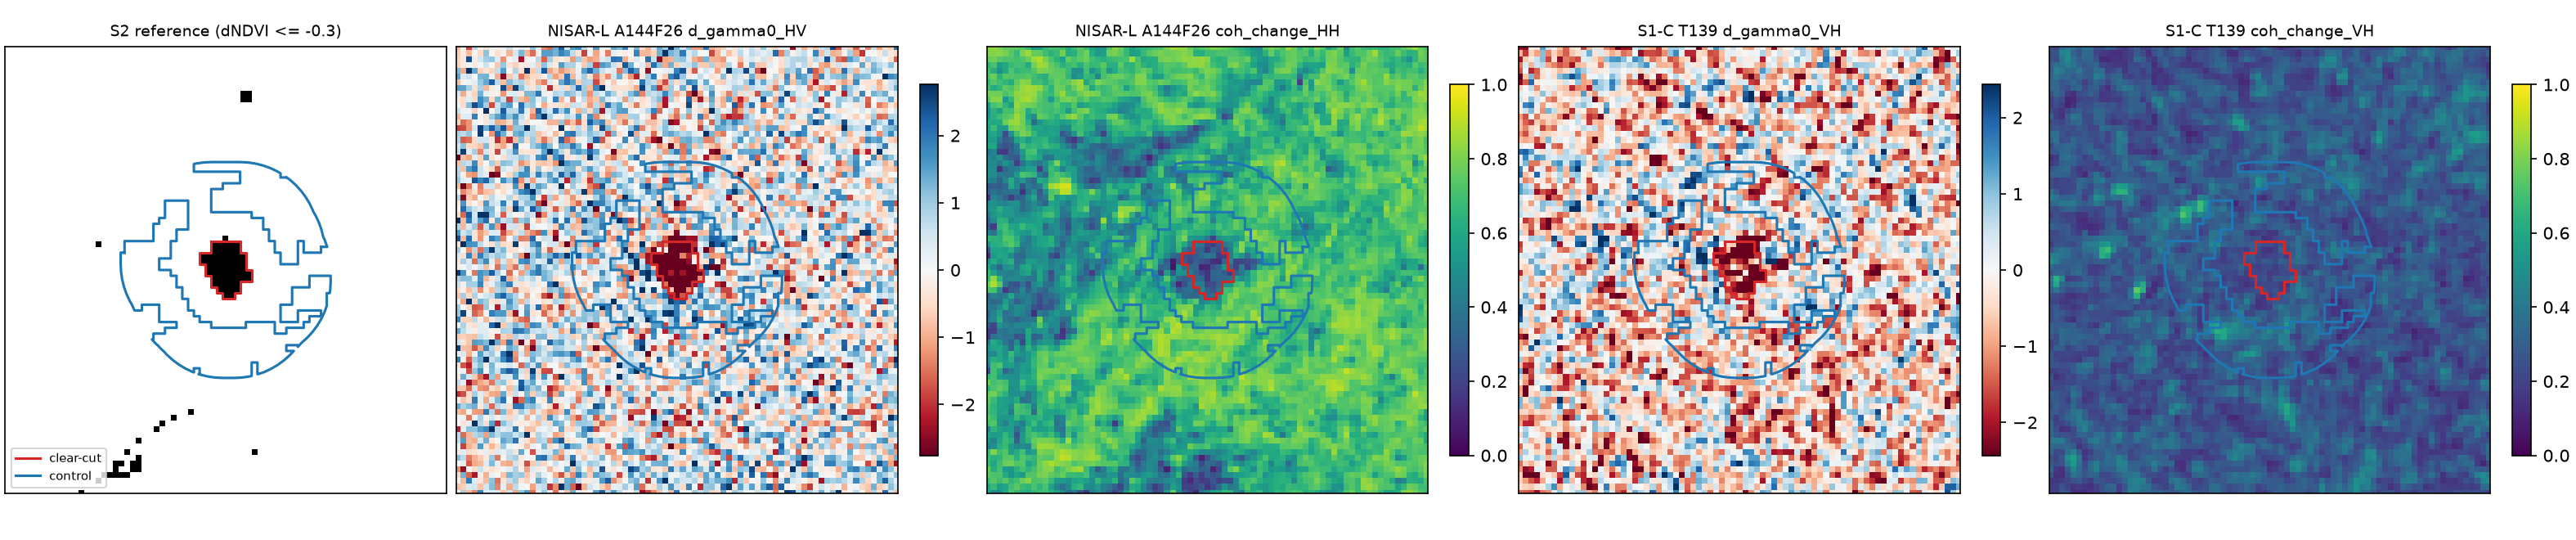
\includegraphics[width=\linewidth]{comparison_maps.png}
\caption{Cartes autour du site. De gauche à droite : référence Sentinel-2, $\Delta\gamma^0$ HV et cohérence de la
paire à cheval NISAR A144, $\Delta\gamma^0$ VH et cohérence de la paire à cheval Sentinel-1. Rouge : coupe ; bleu :
témoin.}
\label{fig-maps}
\end{figure}

\subsection{Sensibilité}

Avec les polygones érodés de 20~m, toutes les séparabilités augmentent :
\begin{itemize}
\item $\Delta\gamma^0$ HV A144 : AUC de 0,97 à 0,996 ;
\item cohérence de la paire à cheval A144 : de 0,995 à 0,999 ;
\item $\gamma^0$ VH Sentinel-1 après : de 0,91 à 0,98 ;
\item cohérence Sentinel-1 : de 0,74 à 0,80 seulement.
\end{itemize}
Les conclusions ne dépendent donc pas des pixels de bordure, et l'écart entre bandes L et C en cohérence demeure.

\subsection{Bilan des hypothèses}

\begin{table}[htbp]
\centering\small
\caption{Bilan des hypothèses du cadrage sur le site C11.}
\label{tab-hyp}
\begin{tabular}{lp{9.3cm}l}
\toprule
& Constat & Verdict \\
\midrule
H1 & Cohérence de la forêt à 12~j : 0,64--0,70 en L contre 0,28 en C. Même à 24~j, elle vaut 0,69 en L. & confirmée \\
H2 & Cohérence de la paire sur la coupe : AUC 0,995 en L contre 0,71--0,74 en C. & confirmée \\
H3 & $\Delta\gamma^0$ croisé : $-4{,}3$~dB (L) contre $-2{,}2$~dB (C) ; contraste persistant en L, transitoire en C. & confirmée \\
H4 & En L, HV $\geq$ HH dans les trois géométries (AUC 0,97 / 0,96, 0,94 / 0,92, 0,84 / 0,72). La cohérence (HH)
fait toutefois encore mieux. & confirmée, à nuancer \\
\bottomrule
\end{tabular}
\end{table}

%=====================================================================
\section{Discussion}

\paragraph{Interprétation physique.} Les résultats sont cohérents avec la longueur d'onde.
\begin{itemize}
\item \textbf{Bande L} (24~cm) : elle traverse le feuillage et interagit avec les troncs et les grosses branches.
  La forêt reste donc cohérente sur 12 à 24~jours, et sa rétrodiffusion HV, dominée par la diffusion de volume,
  chute fortement quand les arbres sont abattus et évacués.
\item \textbf{Bande C} (5,6~cm) : elle interagit surtout avec les feuilles et les rameaux, qui bougent avec le vent.
  La décorrélation temporelle est forte même sans coupe~\cite{zebker1992decorrelation}, ce qui explique la faible
  valeur de la cohérence en bande C pour cet usage.
\item \textbf{Persistance} : la bande C est plus sensible à la rugosité et à l'humidité de surface. À l'automne, le
  sol nu humide et les rémanents de la coupe rediffusent assez pour égaler la forêt, alors que la bande L, moins
  sensible à ces petites structures, conserve le contraste.
\end{itemize}
Pour un suivi opérationnel, cette persistance est un atout majeur. Une coupe reste détectable en bande L des mois
après l'événement, même si une acquisition est manquée.

\paragraph{Dépendance aux conditions.} La cohérence est fortement modulée par la météo.
\begin{itemize}
\item Sur la paire NISAR du 28/09 au 10/10, la cohérence tombe à environ 0,3 dans la forêt comme dans la coupe,
  probablement à cause de la pluie ou du vent.
\item Une détection fondée sur la cohérence doit donc comparer chaque paire à un témoin forestier de la même paire,
  comme ici, plutôt qu'appliquer un seuil absolu.
\end{itemize}

\paragraph{Géométrie d'acquisition.} Les deux géométries montantes (A144, A72) séparent mieux que la descendante
(D138). Sur un relief marqué, l'effet de bord et d'ombre d'une coupe dépend de la direction de
visée~\cite{bouvet2018shadow}. La combinaison de plusieurs géométries, possible avec NISAR, est donc souhaitable.

\paragraph{Complémentarité des deux bandes.} La revisite de Sentinel-1 date la coupe plus finement.
\begin{itemize}
\item Le 02/08, aucun changement n'est visible en bande C (AUC VH 0,57) ; le 14/08, il est net. L'essentiel de
  la coupe a donc eu lieu entre le 2 et le 11~août, ce qui est cohérent avec le NDVI.
\item Le système le plus robuste combinerait la bande C pour la réactivité et la bande L pour la confirmation et la
  persistance.
\end{itemize}

\paragraph{Limites.}
\begin{enumerate}
\item \textbf{Un seul site} de 2,4~ha. Les intervalles de confiance traduisent la variabilité entre pixels, pas
  entre sites ; il faut répliquer sur plusieurs coupes (le candidat C09 est disponible).
\item La paire NISAR sur la coupe fait \textbf{24~jours} contre 12 pour Sentinel-1. Cela défavorise la bande L, ce
  qui renforce la conclusion.
\item Les produits NISAR sont \textbf{provisoires} (2026), et peu de paires sont disponibles avant la coupe
  (1 à 3).
\item À 80~m, la coupe ne contient qu'environ 4 pixels indépendants. Les AUC égales à 1 de la couche
  \texttt{coh80} sont donc indicatives.
\item Le F1 de détection est bas, en raison de la très faible prévalence et du seuillage d'une seule variable. Une
  détection opérationnelle demanderait :
  \begin{itemize}
  \item une combinaison de variables ($\gamma^0$ HV et cohérence) ;
  \item un filtrage spatial (taille minimale d'objet) ;
  \item une confirmation sur plusieurs dates.
  \end{itemize}
\item Le dépérissement (scolytes) est fréquent dans la zone. Sa signature radar, différente d'une coupe, n'a pas été
  étudiée ici.
\end{enumerate}

%=====================================================================
\section{Chaîne réutilisable et perspectives}

\paragraph{Une chaîne réutilisable.} Le traitement est organisé en un paquet Python importable
(\texttt{src/nisar\_s1}). Les scripts ne font qu'orchestrer :
\begin{itemize}
\item lecture des produits NISAR L2 d'ISCE3 en local ou à distance (\texttt{io\_nisar}) ;
\item téléchargement partiel (\texttt{download}) ;
\item graphes et pilotage de SNAP (\texttt{snap}) ;
\item grille commune (\texttt{grid}) ;
\item métriques (\texttt{stats}) et détection (\texttt{detect}) ;
\item figures (\texttt{plots}).
\end{itemize}
Les paramètres sont regroupés dans \texttt{config/params.yaml} et les sites en GeoJSON. Changer de site revient à
fournir un nouveau GeoJSON.

\paragraph{Vers ROSE-L.} La mission Copernicus ROSE-L (lancement prévu en 2028~\cite{esa2020rosel}) fournira de la
bande L en Europe dans la continuité de NISAR. La chaîne développée ici repose sur des grandeurs standard : $\gamma^0$ RTC,
cohérence à 12~jours et grille commune. Elle sera transposable en remplaçant le lecteur \texttt{io\_nisar} par un
lecteur des produits ROSE-L. Les produits NISAR étant générés par ISCE3~\cite{isce3}, logiciel ouvert, il est aussi
envisageable de produire avec ISCE3 des produits équivalents à partir des données de niveau~1 des deux missions.

\paragraph{Suites proposées pour le stage.}
\begin{itemize}
\item Réplication sur plusieurs coupes, dont C09, et sur des dépérissements, pour estimer la variabilité entre
  sites.
\item Détecteur multi-variables et multi-géométries ($\gamma^0$ HV et cohérence HH), avec confirmation temporelle et
  validation sur une référence indépendante.
\item Glissements de terrain sous forêt : comparaison des interférogrammes déroulés NISAR et Sentinel-1. La
  cohérence élevée de la bande L en forêt, mise en évidence ici, est précisément ce qui manque à la bande C pour
  l'interférométrie sous couvert.
\item Bande P (BIOMASS) sur des sites tropicaux, puisqu'elle n'acquiert pas en Europe.
\end{itemize}

%=====================================================================
\section{Conclusion}

Sur une coupe rase de 2,4~ha dans les Vosges, la bande L de NISAR se montre nettement plus discriminante que la
bande C de Sentinel-1.
\begin{itemize}
\item \textbf{Cohérence} : la paire qui encadre la coupe sépare presque parfaitement coupe et forêt en bande L
  (AUC 0,995), alors que la bande C n'apporte presque rien (AUC $\approx$ 0,72), la forêt y étant déjà décorrélée.
\item \textbf{Rétrodiffusion} : la chute en polarisation croisée est deux fois plus forte en bande L
  ($-4{,}3$ contre $-2{,}2$~dB).
\item \textbf{Persistance} : le contraste persiste en bande L jusqu'en novembre, alors qu'il disparaît en bande C
  à l'automne.
\end{itemize}
Ces résultats confirment les hypothèses du cadrage et justifient l'intérêt de la bande L pour le suivi des coupes
forestières. Ce suivi pourra être poursuivi avec ROSE-L. Ils devront être consolidés sur davantage de sites avant
de concevoir un détecteur opérationnel.

\printbibliography[heading=bibintoc,title={Références}]

\appendix
%=====================================================================
\section{Reproduction}

Le code est versionné. Les données restent hors du dépôt, sur disque externe. L'environnement conda est
\texttt{environment.yml} ; les identifiants Earthdata sont lus dans \texttt{.netrc}, qui n'est jamais versionné.

\begin{verbatim}
python scripts/02_inventory.py               # inventaire ASF
python scripts/03_site_candidates.py         # candidats (Sentinel-2)
python scripts/03b_verify_candidates.py      # vérification temporelle
python scripts/03c_select_site.py --cand C11 # site et forêt témoin
python scripts/04_fetch_nisar.py             # fenêtres NISAR à distance
python scripts/04_fetch_s1.py --start 2026-06-14 --end 2026-11-07
python scripts/05a_process_s1.py             # SNAP : 13 gamma0 et 12 cohérences
python scripts/05b_compare.py                # comparaison
python scripts/05b_compare.py --erode 20 --tag _erode20
python scripts/06_make_tables.py             # tables LaTeX FR et EN
\end{verbatim}

Les tables de ce rapport sont générées automatiquement à partir des résultats
(\texttt{results/tables/comparison\_*.csv}) : aucun chiffre n'est recopié à la main.

\section{Table complète de séparabilité}

\begin{table}[htbp]
\centering
\scriptsize
\caption{Séparabilité coupe rase / forêt témoin des variables de changement ($\Delta$ : moyenne coupe $-$ moyenne témoin ; $d$ : d de Cohen ; AUC : max(AUC, 1$-$AUC) avec IC par bootstrap par blocs ; JM : Jeffries-Matusita ; AUC fen. et F1$_{max}$ : détection pixel à pixel sur toute la fenêtre, référence dNDVI S2).}
\label{tab-separability}
\begin{tabular}{llcrrlrrr}
\toprule
Capteur & Variable & $n_{av}/n_{ap}$ & $\Delta$ & $d$ & AUC [IC 95\,\%] & JM & AUC fen. & F1$_{max}$ \\
\midrule
NISAR A144F26 & cohérence 80 m, paire sur la coupe HH & 2/6 & $-$0{,}43 & $-$6{,}0 & 1{,}00 [1{,}00--1{,}00] & 1{,}96 & 0{,}88 & 0{,}22 \\
NISAR A144F26 & chute de cohérence 80 m HH & 2/6 & $-$0{,}44 & $-$8{,}7 & 1{,}00 [1{,}00--1{,}00] & 1{,}98 & 0{,}86 & 0{,}33 \\
NISAR A144F26 & chute de cohérence (paire sur la coupe $-$ avant) HH & 2/6 & $-$0{,}42 & $-$4{,}6 & 1{,}00 [0{,}99--1{,}00] & 1{,}82 & 0{,}82 & 0{,}29 \\
NISAR A144F26 & cohérence de la paire sur la coupe HH & 2/6 & $-$0{,}40 & $-$3{,}9 & 1{,}00 [0{,}99--1{,}00] & 1{,}76 & 0{,}87 & 0{,}09 \\
NISAR A144F26 & $\Delta$ cohérence 80 m HH & 2/6 & $-$0{,}08 & $-$2{,}3 & 0{,}98 [0{,}94--1{,}00] & 1{,}35 & 0{,}77 & 0{,}10 \\
NISAR A144F26 & $\gamma^0$ après (dB) HV & 3/8 & $-$4{,}22 & $-$2{,}6 & 0{,}98 [0{,}96--0{,}99] & 1{,}26 & 0{,}93 & 0{,}09 \\
NISAR A144F26 & $\Delta\gamma^0$ après $-$ avant (dB) HV & 3/8 & $-$4{,}25 & $-$3{,}7 & 0{,}97 [0{,}93--0{,}99] & 1{,}28 & 0{,}84 & 0{,}27 \\
NISAR A144F26 & $\Delta\gamma^0$ après $-$ avant (dB) HH & 3/8 & $-$4{,}22 & $-$3{,}2 & 0{,}96 [0{,}93--0{,}99] & 1{,}09 & 0{,}80 & 0{,}24 \\
NISAR A144F26 & $\gamma^0$ après (dB) HH & 3/8 & $-$3{,}34 & $-$2{,}1 & 0{,}95 [0{,}91--0{,}97] & 0{,}94 & 0{,}92 & 0{,}06 \\
NISAR A144F26 & cohérence 80 m après HH & 2/6 & $-$0{,}06 & $-$1{,}4 & 0{,}90 [0{,}81--0{,}97] & 1{,}19 & 0{,}83 & 0{,}03 \\
NISAR A144F26 & $\Delta$ cohérence après $-$ avant HH & 2/6 & $-$0{,}08 & $-$1{,}1 & 0{,}77 [0{,}66--0{,}85] & 0{,}27 & 0{,}67 & 0{,}08 \\
NISAR A144F26 & cohérence après HH & 2/6 & $-$0{,}06 & $-$0{,}9 & 0{,}76 [0{,}65--0{,}85] & 0{,}30 & 0{,}76 & 0{,}02 \\
\addlinespace
NISAR A72F26 & chute de cohérence 80 m HH & 3/5 & $-$0{,}24 & $-$3{,}6 & 1{,}00 [0{,}99--1{,}00] & 1{,}64 & 0{,}76 & 0{,}29 \\
NISAR A72F26 & cohérence 80 m, paire sur la coupe HH & 3/5 & $-$0{,}27 & $-$3{,}3 & 0{,}99 [0{,}98--1{,}00] & 1{,}74 & 0{,}83 & 0{,}24 \\
NISAR A72F26 & $\gamma^0$ après (dB) HV & 3/7 & $-$3{,}56 & $-$2{,}3 & 0{,}96 [0{,}94--0{,}98] & 1{,}12 & 0{,}92 & 0{,}06 \\
NISAR A72F26 & $\Delta\gamma^0$ après $-$ avant (dB) HV & 3/7 & $-$3{,}72 & $-$3{,}0 & 0{,}94 [0{,}89--0{,}99] & 1{,}04 & 0{,}78 & 0{,}27 \\
NISAR A72F26 & $\Delta\gamma^0$ après $-$ avant (dB) HH & 3/7 & $-$2{,}96 & $-$2{,}3 & 0{,}92 [0{,}86--0{,}97] & 0{,}82 & 0{,}78 & 0{,}22 \\
NISAR A72F26 & cohérence de la paire sur la coupe HH & 3/5 & $-$0{,}25 & $-$1{,}8 & 0{,}91 [0{,}85--0{,}96] & 0{,}82 & 0{,}80 & 0{,}07 \\
NISAR A72F26 & chute de cohérence (paire sur la coupe $-$ avant) HH & 3/5 & $-$0{,}22 & $-$1{,}8 & 0{,}88 [0{,}80--0{,}94] & 0{,}62 & 0{,}74 & 0{,}13 \\
NISAR A72F26 & cohérence 80 m après HH & 3/5 & $-$0{,}05 & $-$1{,}3 & 0{,}86 [0{,}72--0{,}93] & 0{,}57 & 0{,}71 & 0{,}02 \\
NISAR A72F26 & $\gamma^0$ après (dB) HH & 3/7 & $-$2{,}35 & $-$1{,}5 & 0{,}85 [0{,}80--0{,}91] & 0{,}47 & 0{,}85 & 0{,}04 \\
NISAR A72F26 & cohérence après HH & 3/5 & $-$0{,}08 & $-$1{,}2 & 0{,}81 [0{,}74--0{,}88] & 0{,}36 & 0{,}71 & 0{,}02 \\
NISAR A72F26 & $\Delta$ cohérence après $-$ avant HH & 3/5 & $-$0{,}05 & $-$0{,}7 & 0{,}65 [0{,}51--0{,}82] & 0{,}15 & 0{,}56 & 0{,}05 \\
NISAR A72F26 & $\Delta$ cohérence 80 m HH & 3/5 & $-$0{,}02 & $-$0{,}5 & 0{,}63 [0{,}51--0{,}80] & 0{,}06 & 0{,}54 & 0{,}01 \\
\addlinespace
NISAR D138F64 & chute de cohérence 80 m HH & 1/5 & $-$0{,}28 & $-$4{,}7 & 1{,}00 [1{,}00--1{,}00] & 1{,}86 & 0{,}86 & 0{,}34 \\
NISAR D138F64 & cohérence 80 m, paire sur la coupe HH & 1/5 & $-$0{,}28 & $-$6{,}8 & 1{,}00 [1{,}00--1{,}00] & 2{,}00 & 0{,}87 & 0{,}08 \\
NISAR D138F64 & cohérence de la paire sur la coupe HH & 1/5 & $-$0{,}31 & $-$3{,}7 & 1{,}00 [0{,}99--1{,}00] & 1{,}72 & 0{,}89 & 0{,}10 \\
NISAR D138F64 & chute de cohérence (paire sur la coupe $-$ avant) HH & 1/5 & $-$0{,}28 & $-$2{,}4 & 0{,}93 [0{,}87--0{,}98] & 0{,}92 & 0{,}81 & 0{,}24 \\
NISAR D138F64 & $\gamma^0$ après (dB) HV & 2/7 & $-$2{,}52 & $-$1{,}5 & 0{,}88 [0{,}81--0{,}94] & 0{,}55 & 0{,}86 & 0{,}05 \\
NISAR D138F64 & cohérence 80 m après HH & 1/5 & $-$0{,}04 & $-$2{,}0 & 0{,}86 [0{,}67--0{,}98] & 0{,}63 & 0{,}60 & 0{,}01 \\
NISAR D138F64 & $\Delta\gamma^0$ après $-$ avant (dB) HV & 2/7 & $-$2{,}33 & $-$1{,}5 & 0{,}84 [0{,}78--0{,}89] & 0{,}44 & 0{,}71 & 0{,}14 \\
NISAR D138F64 & $\gamma^0$ après (dB) HH & 2/7 & $-$1{,}47 & $-$0{,}8 & 0{,}73 [0{,}63--0{,}86] & 0{,}16 & 0{,}75 & 0{,}04 \\
NISAR D138F64 & $\Delta\gamma^0$ après $-$ avant (dB) HH & 2/7 & $-$1{,}69 & $-$1{,}1 & 0{,}72 [0{,}60--0{,}84] & 0{,}29 & 0{,}64 & 0{,}11 \\
NISAR D138F64 & $\Delta$ cohérence 80 m HH & 1/5 & $-$0{,}04 & $-$0{,}7 & 0{,}69 [0{,}51--0{,}89] & 0{,}12 & 0{,}63 & 0{,}02 \\
NISAR D138F64 & cohérence après HH & 1/5 & $-$0{,}03 & $-$0{,}7 & 0{,}68 [0{,}52--0{,}85] & 0{,}13 & 0{,}62 & 0{,}02 \\
NISAR D138F64 & $\Delta$ cohérence après $-$ avant HH & 1/5 & $-$0{,}01 & $-$0{,}1 & 0{,}55 [0{,}50--0{,}67] & 0{,}05 & 0{,}54 & 0{,}03 \\
\addlinespace
Sentinel-1 T139 & $\gamma^0$ après (dB) VH & 4/8 & $-$2{,}27 & $-$1{,}7 & 0{,}91 [0{,}86--0{,}95] & 0{,}67 & 0{,}86 & 0{,}04 \\
Sentinel-1 T139 & $\Delta\gamma^0$ après $-$ avant (dB) VH & 4/8 & $-$2{,}20 & $-$2{,}1 & 0{,}91 [0{,}85--0{,}94] & 0{,}72 & 0{,}79 & 0{,}14 \\
Sentinel-1 T139 & $\Delta\gamma^0$ après $-$ avant (dB) VV & 4/8 & $-$2{,}53 & $-$2{,}4 & 0{,}90 [0{,}82--0{,}95] & 0{,}76 & 0{,}87 & 0{,}22 \\
Sentinel-1 T139 & $\gamma^0$ après (dB) VV & 4/8 & $-$1{,}92 & $-$1{,}5 & 0{,}88 [0{,}82--0{,}92] & 0{,}51 & 0{,}86 & 0{,}04 \\
Sentinel-1 T139 & cohérence de la paire sur la coupe VH & 3/7 & $-$0{,}06 & $-$0{,}8 & 0{,}74 [0{,}68--0{,}80] & 0{,}40 & 0{,}67 & 0{,}01 \\
Sentinel-1 T139 & cohérence après VV & 3/7 & 0{,}04 & 0{,}9 & 0{,}74 [0{,}63--0{,}81] & 0{,}18 & 0{,}68 & 0{,}02 \\
Sentinel-1 T139 & cohérence de la paire sur la coupe VV & 3/7 & $-$0{,}06 & $-$0{,}8 & 0{,}71 [0{,}60--0{,}80] & 0{,}17 & 0{,}63 & 0{,}04 \\
Sentinel-1 T139 & $\Delta$ cohérence après $-$ avant VV & 3/7 & 0{,}06 & 0{,}7 & 0{,}70 [0{,}59--0{,}78] & 0{,}13 & 0{,}66 & 0{,}02 \\
Sentinel-1 T139 & $\Delta$ cohérence après $-$ avant VH & 3/7 & 0{,}03 & 0{,}5 & 0{,}65 [0{,}55--0{,}73] & 0{,}11 & 0{,}61 & 0{,}01 \\
Sentinel-1 T139 & chute de cohérence (paire sur la coupe $-$ avant) VV & 3/7 & $-$0{,}04 & $-$0{,}4 & 0{,}63 [0{,}52--0{,}74] & 0{,}08 & 0{,}57 & 0{,}01 \\
Sentinel-1 T139 & chute de cohérence (paire sur la coupe $-$ avant) VH & 3/7 & $-$0{,}03 & $-$0{,}3 & 0{,}61 [0{,}53--0{,}69] & 0{,}15 & 0{,}59 & 0{,}01 \\
Sentinel-1 T139 & cohérence après VH & 3/7 & 0{,}01 & 0{,}2 & 0{,}55 [0{,}50--0{,}65] & 0{,}02 & 0{,}57 & 0{,}01 \\
\bottomrule
\end{tabular}
\end{table}


\end{document}
